%
%
%   Rodrigo de Marca Françca
% 	rodmarfran@gmail.com / rodrigo.franca@maua.br
%  		
%   Entregavel HW V01
%
% 
%	Maio de 2017

% ------------------------------------------------------------------------
% Projeto de pesquisa - FAPESP
%
% Modelo criado por: Rodrigo Romano
% "Rodrigo A. Romano" <rromano@maua.br>
%
% Alteraćoes: Rafael Corsi
% "Rafael Corsi" <corsiferrao@gmail.com>
% 
% ------------------------------------------------------------------------
\documentclass[12pt,a4paper,twoside=semi]{scrreprt}
%\usepackage[a4paper,left=3.5cm,right=1.5cm,top=3cm,bottom=2.5cm]{geometry}

\usepackage[utf8]{inputenc}       %Permite acentuação
\usepackage[T1]{fontenc}
%\usepackage[english]{babel}
\usepackage[portuguese]{babel}
\usepackage[centertags]{amsmath}

% ------------------------------------------------------------------------
\usepackage[automark,headsepline]{scrlayer-scrpage}
\clearpairofpagestyles
\cfoot[\pagemark]{\pagemark}
\lehead{\headmark}
\rohead{\headmark}
\cfoot[\raisebox{-0.5em}{ -- \, \textnormal{\thepage} \, --}]{\raisebox{-0.5em}{ -- \, \textnormal{\thepage} \, --}}
\pagestyle{scrheadings}
%\include{authorpart}
% ------------------------------------------------------------------------

\usepackage{lmodern,
			url,
			hyperref,
			multirow,
			array,
			indentfirst,
			ncccomma,
			pst-node,
			pstricks,
			schemabloc,
			amssymb,
			amsfonts,
			graphicx,
			etoolbox, 
			pdfpages,
			hyperref,
			paralist,
			tabularx,
			pdflscape,
			color,				
			doc,
			vhistory,
			tcolorbox,
			titlepic,
			hyperref}
			
			
\usepackage[titletoc,toc,title]{appendix}
% ------------------------------------------------------------------------
% Reduz espacamento na bibliografia
%\usepackage{natbib}
%\setlength{\bibsep}{0.0pt}

%Matem figura na secção !
%\usepackage[section]{placeins}

% sub figuras
%ajuste do tamanho entre figuras
\usepackage{subfigure}
\setlength\subfigcapmargin{0.8em}

% Fuzz 
\hfuzz1pt % Don't bother to report over-full boxes if over-edge is < 2pt

% Numeração das notas de rodapé 
\renewcommand{\thefootnote}{\fnsymbol{footnote}}

% Different font in captions 
\newcommand{\captionfonts}{\small}

\makeatletter  % Allow the use of @ in command names
\long\def\@makecaption#1#2{%
  \vskip\abovecaptionskip
  \sbox\@tempboxa{{\captionfonts #1: #2}}%
  \ifdim \wd\@tempboxa >\hsize
    {\captionfonts #1: #2\par}
  \else
    \hbox to\hsize{\hfil\box\@tempboxa\hfil}%
  \fi
  \vskip\belowcaptionskip}
\makeatother   % Cancel the effect of \makeatletter

% Espaçamento
\setlength{\parindent}{30pt} \setlength{\parskip}{6pt}
\newlength{\defbaselineskip}
\setlength{\defbaselineskip}{\baselineskip}

\newcommand{\setlinespacing}[1]{\setlength{\baselineskip}{#1 \defbaselineskip}}
% ---
\newcommand{\PreserveBackslash}[1]{\let\temp=\\#1\let\\=\temp}
\let\PBS=\PreserveBackslash %
\def\baselinestretch{1}
\setlinespacing{1.5}
% ------------------------------------------------------------------------

% Alteracões Corsi

% Use the microtype package for better typography
% http://www.khirevich.com/latex/microtype/
%
% activate={true,nocompatibility} - activate protrusion and expansion
% final - enable microtype; use "draft" to disable
% tracking=true, kerning=true, spacing=true - activate these techniques
% factor=1100 - add 10% to the protrusion amount (default is 1000)
% stretch=10, shrink=10 - reduce stretchability/shrinkability (default is 20/20)
\usepackage[activate={true,nocompatibility},
			final,
			tracking=true,
			kerning=true,
			spacing=true,
			factor=1100,
			stretch=10,
			shrink=10]
			{microtype} 

% Possibilita que caracteres saiam da margem p/ melhor caber o texto
\SetProtrusion{encoding={*},
			   family={bch},
			   series={*},size={6,7}}
               {1={ ,750},2={ ,500},3={ ,500},4={ ,500},5={ ,500},
               6={ ,500},7={ ,600},8={ ,500},9={ ,500},0={ ,500}}

\microtypecontext{spacing=nonfrench}
% ------------------------------------------------------------------------
               
% Todo notes
%\usepackage[disable]{todonotes}
\usepackage[colorinlistoftodos]{todonotes}  
\setlength{\marginparwidth}{2cm}
\reversemarginpar             
%\makeatletter\let\chapter\@undefined\makeatother

\newcommand\todoin[2][]{\todo[inline, caption={2do}, #1, color={red!100!green!33}]{
\begin{minipage}{\textwidth-4pt}#2\end{minipage}}}

% ------------------------------------------------------------------------

% Restora contagem da nota a cada pagina
\usepackage{perpage}
\MakePerPage{footnote}

% Qualidade e compressão do pdf
%\pdfminorversion=5
%\pdfcompresslevel=9
%\pdfobjcompresslevel=2

% ------------------------------------------------------------------------
% Possibilita inserir pdf com texto fora do arquivo
% util para figs geradas no inkscape
\newcommand{\executeiffilenewer}[3]{%
\ifnum\pdfstrcmp{\pdffilemoddate{#1}}%
{\pdffilemoddate{#2}}>0%
{\immediate\write18{#3}}\fi%
}

\newcommand{\includesvg}[1]{%
\executeiffilenewer{#1.svg}{#1.pdf}%
{inkscape -z -D --file=./Figs/#1.svg %
--export-pdf=./Figs/#1.pdf --export-latex}%
\input{./figs/#1.pdf_tex}%
}


\usepackage{hyperref}
\usepackage{lettrine}
\usepackage{multirow}
\usepackage{booktabs}
\usepackage{acronym}
\usepackage{tabularx}
\usepackage{multirow}
\usepackage{tikz}
\usepackage{tcolorbox}
\usepackage{mfirstuc}
\usepackage{bytefield}
\usepackage{etoc}
\usepackage{arydshln}
\usepackage{catchfile}
\usepackage{tikz}
\usepackage[utf8]{inputenc}
\usepackage{outlines}
\usepackage{datetime}
\usetikzlibrary{shapes, arrows, automata, positioning, calc}

% Show sections
\setcounter{tocdepth}{4}
\setcounter{secnumdepth}{4}

% ------------------------------------------------------------------------
% http://latexcolor.com/
% cores dos todos

\definecolor{TBC}{rgb}{0.98, 0.91, 0.71}  	%bananamania
\definecolor{Corsi}{rgb}{0.53, 0.66, 0.42}  %
\definecolor{TBC2}{rgb}{0.86, 0.82, 1.0} %lightmauve
\definecolor{darkgray}{rgb}{0.66, 0.66, 0.66}

\definecolor{lightgreen}{rgb}{0.86, 1, 0.86}
\definecolor{magnolia}{rgb}{0.97, 0.96, 1.0}
\definecolor{maize}{rgb}{0.98, 0.93, 0.37}

\definecolor{babypink}{rgb}{0.96, 0.76, 0.76}

\definecolor{citrine}{rgb}{0.89, 0.82, 0.04}

\definecolor{darkorange}{rgb}{1.0, 0.55, 0.0}


\definecolor{colorOK}{rgb}{0.56, 0.74, 0.56}
\definecolor{anti-flashwhite}{rgb}{0.95, 0.95, 0.96}
\definecolor{colorIMP}{rgb}{0.89, 0.85, 0.44}
\definecolor{colorNO}{rgb}{0.97, 0.97, 1.0}
\definecolor{ghostwhite}{rgb}{0.97, 0.97, 1.0}

\newcommand\crule[3][black]{\textcolor{#1}{\rule{#2}{#3}}}

\newcounter{myexample}

\newtcolorbox[	use counter=myexample]
				{ReqOK}[2][]{%
				colback=ghostwhite,
				colframe=colorOK,
				coltitle=black,
				fonttitle=\bfseries,
				title=REQ SIMUCAM - \thetcbcounter: \capitalisewords{#2}}

\newtcolorbox[	use counter=myexample]
				{ReqIMP}[2][]{%
				colback=ghostwhite,
				colframe=colorIMP,
				coltitle=black,
				fonttitle=\bfseries,
				title=REQ SIMUCAM - \thetcbcounter: \capitalisewords{#2}}
			
\newtcolorbox[	use counter=myexample]
				{ReqNO}[2][]{%
				colback=ghostwhite,
				colframe=colorNO,
				coltitle=black,
				fonttitle=\bfseries,
				title=REQ SIMUCAM - \thetcbcounter: \capitalisewords{#2}}
			
\newtcolorbox[	use counter=myexample]
				{QUESTION}[2][]{%
				colback=ghostwhite,,
				colframe=darkgray,
				coltitle=black,				
				fonttitle=\bfseries,
				title=REQ SIMUCAM - \thetcbcounter: \capitalisewords{#2}}
		
% ------------------------------------------------------------------------

\newcommand{\RF}{Rodrigo França}

\newcommand{\LastUpdateVersion}{1.0.0}
\newcommand{\LastUpdateDate}{23/06/2017}
\newcommand{\LastUpdateDateLong}{23 de Junho de 2017}

\newcommand{\addrevisiontable}{
  \begin{center}
  	\begin {tabularx}{\textwidth}{l l l X}
  	\textbf{Revisão} & \textbf{Data} & \textbf{Autor(es)} & \textbf{Descrição}\\ \hline
  	\LastUpdateVersion & 
  	\shortdate \LastUpdateDate & 
  	\RF & 
  	Criação do documento. \\
  	\end {tabularx}
  \end{center}
}

% ------------------------------------------------------------------------

%\titlehead	{\flushright 
\includegraphics[width=0.3\linewidth]{./maua_logo}}
\title		{   \LARGE
				Instituto Mauá de Tecnologia \\
				Núcleo de Sistemas Eletrônicos Embarcados - NSEE \\ 
				\huge 
				\vspace{12px}
				MEB - SIMUCAM X \\
				Hardware FTDI - USB 3.0 \\
				V. \LastUpdateVersion
			}
\author		{
			 Rodrigo França \\ \small 	
			 \href{mailto:rodrigo.franca@maua.com}{rodrigo.franca@maua.com}
			% \vspace{10px}\\
			% Vanderlei Parro \\ \small 	
			%\href{mailto:vparro@mac.com}{vparro@mac.com}
			}
%\subject	{Núcleo de Sistemas Eletrônicos Embarcados - NSEE}			
\titlepic	{
\includegraphics[width=0.4\textwidth]{maua_logo}}
\date       {\LastUpdateDateLong}

\renewcommand{\contentsname}{Whatever}

% ------------------------------------------------------------------------
% Inicio
% ------------------------------------------------------------------------
\begin{document}

\maketitle
\tableofcontents

% ------------------------------------------------------------------------

\chapter*{Revisões}
\addcontentsline{toc}{chapter}{Revisões}
\addrevisiontable

\chapter{Introdução}

  \section{Objetivo}
    O objetivo deste documento é descrever o hardware implementado para a utilização do módulo FTDI UMFT601A, assim como o firmware necessário para utilizá-lo. A utilização do módulo UMFT601A, por sua vez, tem o objetivo de permitir a comunicação entre a MEB (FPGA) e o PC embarcado (NUC), através de uma interface USB 3.0.

  \section{Escopo}
    O escopo deste documento é:
    \begin{enumerate}
    	\item Descrição do hardware implementado para comunicação entre módulo UMFT601A e o microprocessador NIOS II;
    	\item Descrição do firmware utilizado para comunicação com o Hardware descrito no item 1;
    	\item Apresentação de outros sistemas presentes na MEB que podem interagir com o Hardware descrito no item 1 (memórias DDR2, DMA, etc.);
    	\item Apresentar o ambiente de programação e debug do microcontrolador presente na MEB;
    	\item Apresentar uma lista de documentos e links interessantes para desenvolvimento com o módulo UMFT601A.
    \end{enumerate}
  
\chapter{Hardware}

  \section{Introdução}
    Para a utilização do módulo UMFT601A, foi desenvolvido um componente de hardware responsável pelo acesso físico aos pinos do módulo. Esse componente foi denominado “FTDI” e foi integrado ao sistema da MEB através do ambiente Qsys. Um diagrama de blocos geral é apresentado na figura \ref{fig:general}.
    
  \section{Implementação}
    O componente “FTDI” serve apenas como uma conexão física entre os pinos do módulo UMFT601A e o microprocessador NIOS II, não realizando nenhuma lógica especifica. O objetivo é, inicialmente, que essa lógica seja implementada em firmware para depois ser recriada em hardware.
    O módulo possui:
    \begin{itemize}
    	\item Interface com o barramento Avalon (utilizado pelo NIOS II), para escrita e leitura de seus registradores;
    	\item Registradores para acessar e controlar os pinos do módulo UMFT601A (registradores descritos na tabela \ref{tab:reg_ftdi}). Maiores informações podem ser encontradas no arquivo "FTDI\_Registers.ods", dentro da pasta "Referências", dentro de "Implementation";
    	\item Interface externa com os pinos do módulo UMFT601A (interface descrita na tabela \ref{tab:interface_ftdi}).
    	O desenho do módulo “FTDI” pode ser visto na figura \ref{fig:component_ftdi}. Maiores informações podem ser encontradas no arquivo "Pin\_Mapping.ods", dentro da pasta "Referências", dentro de "Implementation"
    \end{itemize}
    \bigskip
   
  \begin{figure}[htpb]
  \centering 
	\resizebox{\textwidth}{!}{
	  \begin{tikzpicture}[>=stealth',shorten >=1pt, auto,node distance=3cm, square/.style={regular polygon,regular polygon sides=4, inner sep=-2pt}]
		
		\node[square, minimum height=3cm, draw, align=center] (NIOS) {NIOS II};
		\node[rectangle, minimum height=4cm, above right=of NIOS, draw, align=center] (M1) {DDR2 M1};
		\node[rectangle, minimum height=4cm, below right=of NIOS, draw, align=center] (M2) {DDR2 M2};
		\node[rectangle, minimum height=1cm, draw, align=center] at ($(M1)!0.5!(M2)$) (DMA) {DMA};
		\node[rectangle, above left=of NIOS, align=center] (JTAG) {JTAG/UART};
		\node[rectangle, below left=of NIOS, align=center] (DISP) {7-SEG DISPLAY \\ PAINEL LEDS};
		\node[rectangle, left=1.5cm of DISP, align=center] (TEMP) {TEMPERATURE \\ SENSOR};
		\node[rectangle, left=2.4cm of JTAG, align=center, font=\bf] (FTDI) {UMFT601A \\ USB 3.0};
		
		\path[<->] (NIOS) edge [bend left=40] node {data} (M1);
		\path[<->] (NIOS) edge [bend right=40] node {data} (M2);
		\path[<->] (NIOS) edge node {commands} (DMA);
		\path[<->, dashed] (DMA) edge node {data} (M1);
		\path[<->, dashed] (DMA) edge node {data} (M2);
		\path[<->] (NIOS) edge node {usb} (JTAG);
		\path[<-] (NIOS) edge node {i2c} (TEMP);
		\path[->] (NIOS) edge node {bus} (DISP);
		\path[<->, font=\bf] (NIOS) edge node {avalon bus} (FTDI);
		
	  \end{tikzpicture}
	}
	\caption{Diagrama de Blocos geral da MEB}
	\label{fig:general}
    \end{figure}

  	\begin{longtable}{>{\arraybackslash}p{5cm} >{\centering\arraybackslash}p{3cm} >{\centering\arraybackslash}p{6.4cm}}
  		\caption{Registradores do Componente "FTDI"{}} \label{tab:reg_ftdi}  \medskip \\
  		\centering\textbf{Registrador} & \textbf{Endereço} & \textbf{Descrição} \\
\hline
\endfirsthead
\multicolumn{3}{c}%
{\tablename\ \thetable\ -- \textit{Continuação da página anterior}} \\
\hline
\textbf{Registrador} & \textbf{Endereço} & \textbf{Descrição} \\
\hline
\endhead
\hline \multicolumn{3}{r}{\textit{Continua na proxima página}} \\
\endfoot
\endlastfoot

    DATA\_REG\_IN & 0x00000000 (Leitura) & Registro com o valor de entrada do barramento DATA (caso DATA\_OE = ‘0’) \\
    DATA\_REG\_OUT & 0x00000000 (Escrita) & Registro com o valor de saída do barramento DATA (caso DATA\_OE = ‘1’) \\
    BE\_REG\_IN & 0x00000001 (Leitura) & Registro com o valor de entrada do barramento BE (caso BE\_OE = ‘0’) \\
    BE\_REG\_OUT & 0x00000001 (Escrita) & Registro com o valor de saída do barramento BE (caso BE\_OE = ‘1’) \\
    TXE\_N\_REG & 0x00000002 & Registro com o valor de entrada do pino TXE\_N \\
    RXF\_N\_REG & 0x00000003 & Registro com o valor de entrada do pino RXF\_N \\
    SIWU\_N\_REG & 0x00000004 & Registro com o valor de saída do pino SIWU\_N \\
    WR\_N\_REG & 0x00000005 & Registro com o valor de saída do pino WR\_N \\
    RD\_N\_REG & 0x00000006 & Registro com o valor de saída do pino RD\_N \\
    OE\_N\_REG & 0x00000007 & Registro com o valor de saída do pino OE\_N \\
    RESET\_N\_REG & 0x00000008 & Registro com o valor de saída do pino RESET\_N \\
    WAKEUP\_N\_REG\_IN & 0x00000009 (Leitura) & Registro com o valor de entrada do pino WAKEUP\_N (caso WAKEUP\_OE = ‘0’) \\
    WAKEUP\_N\_REG\_OUT & 0x00000009 (Escrita) & Registro com o valor de saída do pino WAKEUP\_N (caso WAKEUP\_OE = ‘1’) \\
    GPIO\_REG\_IN & 0x0000000A (Leitura) & Registro com o valor de entrada do barramento GPIO (caso GPIO\_OE = ‘0’) \\
    GPIO\_REG\_OUT & 0x0000000A (Escrita) & Registro com o valor de saída do barramento GPIO (caso GPIO\_OE = ‘1’) \\
    OE\_REG & 0x0000000B & Registro para controle dos OE (Output Enable) para os pinos bidirecionais (DATA, BE, WAKEUP, GPIO) \\
    DATA\_OE\_MASK\_REG & 0x0000000C (Escrita) & Registro fantasma para mascarar o sinal DATA\_OE \\
    BE\_OE\_MASK\_REG & 0x0000000D (Escrita) & Registro fantasma para mascarar o sinal BE\_OE \\
    WAKEUP\_OE\_MASK\_REG & 0x0000000E (Escrita) & Registro fantasma para mascarar o sinal WAKEUP\_OE \\
    GPIO\_OE\_MASK\_REG & 0x0000000F (Escrita) & Registro fantasma para mascarar o sinal GPIO\_OE \\

	\end{longtable}


  	\begin{longtable}{>{\centering\arraybackslash}p{4.8cm} >{\centering\arraybackslash}p{4.8cm} >{\centering\arraybackslash}p{4.8cm}}
  	\caption{Interface externa do Componente "FTDI"{}} \label{tab:interface_ftdi}  \medskip \\
    \textbf{Pino UMFT601A} & \textbf{Pino HSMC} & \textbf{Pino FPGA} \\
\hline
\endfirsthead
\multicolumn{3}{c}%
{\tablename\ \thetable\ -- \textit{Continuação da página anterior}} \\
\hline
\textbf{Pino UMFT601A} & \textbf{Pino HSMC} & \textbf{Pino FPGA} \\
\hline
\endhead
\hline \multicolumn{3}{r}{\textit{Continua na proxima página}} \\
\endfoot
\endlastfoot
    60 / D\_CLK  &  40 / CLKIN0  & PIN\_AC34 \\
    9  / RXF\_N  &  104 / D43  & PIN\_AR32 \\
    8  / TXE\_N  &  102 / D41  & PIN\_AP32 \\
    18 / GPIO\_1  &  113 / D48  & PIN\_AD30 \\
    17 / GPIO\_0  &  115 / D50  & PIN\_AD31 \\
    11 / WR\_N  &  110 / D47  & PIN\_AT30 \\
    12 / RD\_N  &  114 / D49  & PIN\_AT33 \\
    13 / OE\_N  &  116 / D51  & PIN\_AU33 \\
    10 / SIWU\_N  &  108 / D45  & PIN\_AR31 \\
    8  / BE\_N\_3  &  109 / D46  & PIN\_AK29 \\
    7  / BE\_N\_2  &  107 / D44  & PIN\_AJ29 \\
    5  / BE\_N\_1  &  103 / D42  & PIN\_AC29 \\
    4  / BE\_N\_0  &  101 / D40  & PIN\_AC28 \\
    76 / DATA31  &  86 / D31  & PIN\_AN31 \\
    75 / DATA30  &  84 / D29  & PIN\_AM31 \\
    74 / DATA29  &  80 / D27  & PIN\_AM35 \\
    73 / DATA28  &  78 / D25  & PIN\_AM34 \\
    72 / DATA27  &  74 / D23  & PIN\_AP30 \\
    71 / DATA26  &  72 / D21  & PIN\_AN30 \\
    70 / DATA25  &  68 / D19  & PIN\_AK35 \\
    69 / DATA24  &  66 / D17  & PIN\_AK34 \\
    67 / DATA23  &  62 / D15  & PIN\_AJ35 \\
    66 / DATA22  &  60 / D13  & PIN\_AJ34 \\
    65 / DATA21  &  56 / D11  & PIN\_AH35 \\
    64 / DATA20  &  54 / D9  & PIN\_AH34 \\
    63 / DATA19  &  50 / D7  & PIN\_AK33 \\
    62 / DATA18  &  48 / D5  & PIN\_AJ32 \\
    61 / DATA17  &  44 / D3  & PIN\_AC32 \\
    60 / DATA16  &  42 / D1  & PIN\_AC31 \\
    57 / DATA15  &  85 / D30  & PIN\_AG32 \\
    56 / DATA14  &  83 / D28  & PIN\_AG31 \\
    55 / DATA13  &  79 / D26  & PIN\_AF26 \\
    54 / DATA12  &  77 / D24  & PIN\_AE26 \\
    53 / DATA11  &  73 / D22  & PIN\_AE29 \\
    52 / DATA10  &  71 / D20  & PIN\_AE28 \\
    51 / DATA9 &  67 / D18  & PIN\_AD29 \\
    50 / DATA8  &  65 / D16  & PIN\_AD28 \\
    47 / DATA7  &  61 / D14  & PIN\_AE27 \\
    46 / DATA6  &  59 / D12  & PIN\_AD27 \\
    45 / DATA5  &  55 / D10  & PIN\_AB31 \\
    44 / DATA4  &  53 / D8  & PIN\_AB30 \\
    43 / DATA3  &  49 / D6  & PIN\_AB28 \\
    42 / DATA2  &  47 / D4  & PIN\_AB27 \\
    41 / DATA1  &  43 / D2  & PIN\_AD26 \\
    40 / DATA0  &  41 / D0  & PIN\_AC26 \\
    15 / RESET\_N  &  119 / D52  & PIN\_AK32 \\
    16 / WAKE\_UP\_N  &  121 / D54  & PIN\_AL32 \\
  	\end{longtable}
  
 
  \begin{figure}[htpb]
  	\centering
    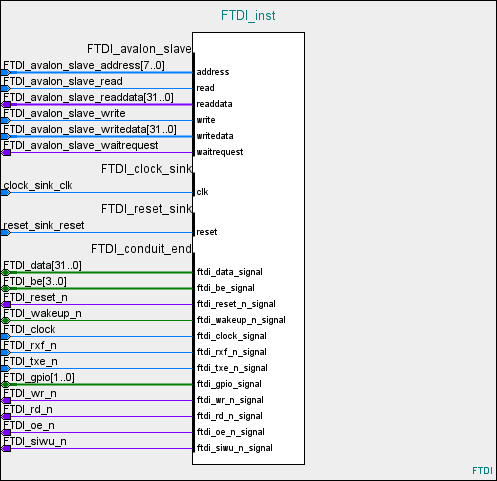
\includegraphics[width=0.8\textwidth]{figs/Componente_FTDI}
  	\caption{Desenho do Componente "FTDI"{}}
  	\label{fig:component_ftdi}
  \end{figure}

\chapter{Firmware}

  \section{Introdução}
    Para acesso aos registradores do módulo “FTDI”, foi desenvolvida uma biblioteca (arquivos “ftdi.h” e “ftdi.c”, presentes na pasta “usb3” dentro da pasta "logic") . Essa biblioteca possui funções básicas para acesso aos registradores do componente “FTDI” e aos pinos do módulo UMFT601A.

  \section{Implementação}
    Foi implementado um total de duas funções, listadas na tabela \ref{tab:list_ftdi}. Maiores informaçõe podem ser enontradas nos arquivos "ftdi.h" e "ftdi.c".
    \bigskip

  \begin{table}[htpb]
  	\centering
  	\begin{tabularx}{\textwidth}{p{4.2cm} X}
  		\centering\arraybackslash\textbf{Nome} & \centering\arraybackslash\textbf{Descrição} \\ \hline
          FTDI\_WRITE\_REG & Realiza a escrita nos registradores do componente “FTDI” (escrita nos pinos do módulo UMFT601A). Recebe o endereço do registrador e o valor a ser escrito; Retorna se a escrita foi bem sucedida ou não.\\
          FTDI\_READ\_REG & Realiza a leitura dos registradores do componente “FTDI” (leitura dos pinos do módulo UMFT601A). Recebe o endereço do registrador; Retorna o valor do registrador.\\
  	\end{tabularx}
  	\caption{Lista de funções para utilizar o Componente "FTDI"{}}
  	\label{tab:list_ftdi}
  \end{table}
  
  
 
\chapter{Outros Sistemas}
  A MEB possui, além do componente “FTDI” e do microprocessador NIOS II, outros componentes e sistemas que podem interagir com o módulo UMFT601A. Entre eles, os principais são:
  \begin{itemize}
  	\item  Controladores de memória DDR2, para duas memórias de 1GB (denominadas “M1” e ”M2”);
  	\item  Controladores de DMA entre as memórias DDR2 (um DMA para transferência de dados de M1 para M2 e outro DMA para transferência de dados de M2 para M1);
  	\item  Controlador para LEDs da placa DE4 e do painel frontal;
  	\item  Controlador para o display de sete segmentos da placa DE4;
  	\item  Comunicação UART com o computador através de cabo USB;
  	\item  Comunicação JTAG para gravação e debug do microcontrolador.
  \end{itemize}
  \medskip
  Não é do escopo deste documento fornecer descrição de como esses outros sistemas funcionam. Existem bibliotecas prontas para a utilização deles, e serão fornecidas.

\chapter{Programação}
  A programação do microcontrolador é realizado através de um cabo USB, conectado a uma interface JTAG na placa DE4. O ambiente de programação é uma versão modificada do Eclipse, fornecido pela Altera junto com o software Quartus. Para realizar os testes é necessário gravar, pelo Quartus, o hardware de testes e então programar a MEB (microcontrolador) com o Eclipse.
  Embora exista um software para simulação de hardware (ModelSim, que é fornecido com o Quartus), não é possível simular o módulo FTDI ou uma interface USB 3.0. Dessa forma, se faz necessária a utilização física da MEB para qualquer teste de maior complexidade.
  
\chapter{Referências}
  \begin{itemize}
  	\item Website do módulo UMFT601A (\url{http://www.ftdichip.com/Products/Modules/SuperSpeedModules.htm})
  	\item Datasheet do módulo UMFT601A (\url{http://www.ftdichip.com/Support/Documents/DataSheets/Modules/DS_UMFT60xx%20module%20datasheet.pdf})
  	\item Website do componente FT601Q (\url{http://www.ftdichip.com/Products/ICs/FT600.html})
  	\item Datasheet do componente FT601Q (\url{http://www.ftdichip.com/Support/Documents/DataSheets/ICs/DS_FT600Q-FT601Q%20IC%20Datasheet.pdf})
  	\item Application Note AN370 - FT60X Configuration Programmer User Guide (\url{http://www.ftdichip.com/Support/Documents/AppNotes/AN_370%20FT600%20Configuration%20Programmer%20User%20Guide.pdf})
  	\item Application Note AN375 - FT600 Data Loopback Application User Guide (\url{http://www.ftdichip.com/Support/Documents/AppNotes/AN_375%20FT600%20Data%20Loopback%20Application%20User%20Guide.pdf})
  	\item Application Note AN377 - Altera FPGA FIFO master Programming Guide (\url{http://www.ftdichip.com/Support/Documents/AppNotes/AN_377%20Altera%20FPGA%20FIFO%20master%20Programming%20Guide.pdf})
  	\item Application Note AN379 - D3XX Programmers Guide (\url{http://www.ftdichip.com/Support/Documents/ProgramGuides/AN_379%20D3xx%20Programmers%20Guide.pdf})
  	\item Application Note AN386 - FT600 Maximize Performance (\url{http://www.ftdichip.com/Support/Documents/AppNotes/AN_386%20FTDI%20FT600%20Maximize%20Performance.pdf})
  	\item Application Note AN387 - FT600 Data Streamer Application User Guide (\url{http://www.ftdichip.com/Support/Documents/AppNotes/AN_387%20FT600%20Data%20Streamer%20Application%20User%20Guide.pdf})
  	\item Application Note AN421 - FIFO Bus Master for FT60x (\url{http://www.ftdichip.com/Support/Documents/AppNotes/AN_421_FIFO_Bus_Master_For%20FT60x.pdf})
  \end{itemize}

\end{document}


